\documentclass[reqno]{amsart}
\usepackage{amsfonts,amsmath,amsthm,amssymb,latexsym, cite}%
\usepackage{graphicx,verbatim}
\usepackage[colorlinks,plainpages,citecolor=magenta, linkcolor=blue ]{hyperref}%,bookmarksnumbered,, backref

\theoremstyle{plain}
\newtheorem{thm}{Theorem}
\newtheorem*{thrm}{Theorem}
\newtheorem{defn}{Definition}
\newtheorem{cor}{Corollary}
\newtheorem{lem}{Lemma}
\newtheorem{rem}{Remark}
\newtheorem{prop}{Proposition}


\textwidth=125mm
\textheight=195mm

\numberwithin{equation}{section}


\newcommand{\dom}{\mathop{\rm dom}}
\renewcommand{\Im}{\mathop{\rm Im}}
\newcommand{\supp}{\mathop{\rm supp}}
\newcommand{\sgn}{\mathop{\rm sgn}}
\newcommand{\rank}{\mathop{\rm rank}}
\renewcommand{\kappa}{\varkappa}
\newcommand{\rmi}{{\rm i}}
\newcommand{\Real}{\mathbb R}
\newcommand{\Cmpl}{\mathbb C}
\newcommand{\eps}{\varepsilon}
\newcommand{\en}{{\nu,\eps}}
\newcommand{\cI}{\mathcal{I}}
\newcommand{\cF}{\mathcal{F}}
\newcommand{\mv}[1]{\langle #1 \rangle_0}
\newcommand{\fm}[1]{\langle #1 \rangle_1}
\newcommand{\fpr}[1]{{#1}^{(-1)}}
\newcommand{\spr}[1]{{#1}^{(-2)}}
\newcommand{\ra}{\rangle}
\newcommand{\la}{\langle}
\newcommand{\fra}{\mathfrak{a}}

% MATH -----------------------------------------------------------
\newcommand{\norm}[1]{\left\Vert#1\right\Vert}
\newcommand{\abs}[1]{\left\vert#1\right\vert}
\newcommand{\set}[1]{\left\{#1\right\}}
\newcommand{\To}{\longrightarrow}
\newcommand{\BX}{\mathbf{B}(X)}
\newcommand{\A}{\mathcal{A}}
\newcommand{\cH}{\mathcal{H}}
\newcommand{\cV}{\mathcal{V}}
% ----------------------------------------------------------------

\newcommand{\mg}[1]{{\color{magenta}{#1}}}
\newcommand{\rd}[1]{{\color{red}{#1}}}
\renewcommand{\emph}[1]{{\textit{#1}}}
%\renewcommand{\phi}{\varphi}
\newcommand\rmd{\mathrm{d}}
\newcommand\rme{\mathrm{e}}
\newcommand\rmR{\mathrm{R}}
\renewcommand{\leq}{\leqslant}
\renewcommand{\geq}{\geqslant}
\newcommand{\myIm}{\mathop{\rm Im}}
\newcommand{\myRe}{\mathop{\rm Re}}
\newcommand{\sign}{\mathop{\rm sign}}
\newcommand{\ess}{\mathop{\rm ess}}
\newcommand{\bl}[1]{{\color{blue}{#1}}}
\newcommand{\oB}[1]{\langle{#1},g\rangle\hskip1pt f+\langle{#1},f\rangle\hskip1pt g}
\newcommand\nep{\textstyle\frac r\eps}
\newcommand\te{\left(\frac t\eps\right)}
\newcommand\se{\left(\frac s\eps\right)}
\newcommand\pfg{p}
\newcommand\hy{\hat{y}_\eps}
\newcommand{\pte}{\partial_n}
\newcommand{\pts}{\partial_s}
\newcommand{\npt}{\partial_\nu}

\begin{document}





\title[Schr\"{o}dinger operators with a $(a\partial_\nu\delta_\gamma+b\delta_\gamma)$-like potentials]
{Schr\"{o}dinger operators with a $(a\partial_\nu\delta_\gamma+b\delta_\gamma)$-like potentials}





\author{Yuriy Golovaty}%
\address{Department of Mechanics and Mathematics,
  Ivan Franko National University of Lviv\\
  1 Universytetska str., 79000 Lviv, Ukraine}
\email{yuriy.golovaty@lnu.edu.ua}

\subjclass[2000]{Primary 34L40, 34B09; Secondary  81Q10}


\begin{abstract}
The
\end{abstract}


\keywords{}
\maketitle





%%%%%%%%%%%%%%%%%%%%%%%%%%%%%%%%%%%%%%%%%%%%%%%%%%%%%%%%%%%%%%%%%%%%%%%%%%
% Introduction
%%%%%%%%%%%%%%%%%%%%%%%%%%%%%%%%%%%%%%%%%%%%%%%%%%%%%%%%%%%%%%%%%%%%%%%%%%

\section{Introduction  }
\label{Sec:Introduction}




Throughout the paper, $W_2^m(\Omega)$ stands for the Sobolev space of functions defined on a set $\Omega$.







%%%%%%%%%%%%%%%%%%%%%%%%%%%%%%%%%%%%%%%%%%%%%%%%%%%%%%%%%%%%%%%%%%%%%%%%%%
% Statement of Problem and Main Results
%%%%%%%%%%%%%%%%%%%%%%%%%%%%%%%%%%%%%%%%%%%%%%%%%%%%%%%%%%%%%%%%%%%%%%%%%%

\section{Statement of Problem and Main Results}
\label{Sec:Statment}

Let us consider the family of operators
\begin{equation}\label{OprHe}
H_\eps=-\Delta +W+V_\eps,
\end{equation}
where the potential $W$ increases as $|x|\to +\infty$ and $W\in L^\infty_{loc}(\Real^2)$. We define the potential $V_\eps$ as follows.
Let $\gamma$ be a  closed $C^3$-curve without self-intersection
points. We will denote by $\omega_\eps$ the $\eps$-neighborhood of $\gamma$, i.e., the union of all open balls with radius $\eps$ and center on~$\gamma$.  Suppose that $V_\eps$ has a compact support that lies  in $\omega_\eps$ and  shrinks to $\gamma$ as $\eps\to 0$. To specify  the dependence of $V_\eps$ on  small parameter $\eps$ we introduce  curvilinear coordinates coordinates in $\omega_\eps$. Let $S$ be the circle of the same length as the length of $\gamma$. We will parameterize $\gamma$ by points of the circle.
Let $\alpha\colon\; S\to \Real^2$ be the unit-speed $C^3$-parametrization of $\gamma$ with the natural parameter $s\in S$.
Then $\nu=(-\dot{\alpha}_2, \dot{\alpha}_1)$ is a unit normal on $\gamma$, because  $\dot{\alpha}_1^2+\dot{\alpha}_2^2=1$.
We define the local coordinates $(s,r)$ in $\omega_\eps$ by
\begin{equation}\label{LocalTr}
    x=\alpha(s)+r\nu(s), \qquad (s,r)\in Q_\eps=S\times (-\eps, \eps).
\end{equation}
The coordinate $r$ is the signed distance from a point $x$ to $\gamma$.
Therefore  $\omega_\eps$ is diffeomorphic to cylinder $Q_\eps$ for $\eps$ small enough. Suppose that the localized potential $V_\eps$ has the following structure
\begin{equation}\label{Veps}
V_\eps\big(\alpha(s)+r\nu(s)\big)=\eps^{-2}\,V\left(\eps^{-1}r\right)
+\eps^{-1}\,U\left(s,\eps^{-1}r\right),
\end{equation}
where $V$ and $U$ are measurable bounded functions such that the supports
of $V$ and $U(s,\,\cdot\,)$ lie in $\cI=(-1,1)$ for all $s\in S$.
The key assumption is that $V$ does not depend on  $s$.
Note that the unperturbed operator $H_0=-\Delta +W$ is self-adjoint in $L^2(\Real^2)$, its domain is a part of $W_{2,loc}^2$,  and the spectrum of $H_0$ is discrete.  Obviously, we have $\dom H_\eps=\dom H_0$.

\begin{figure}[b]
\centering
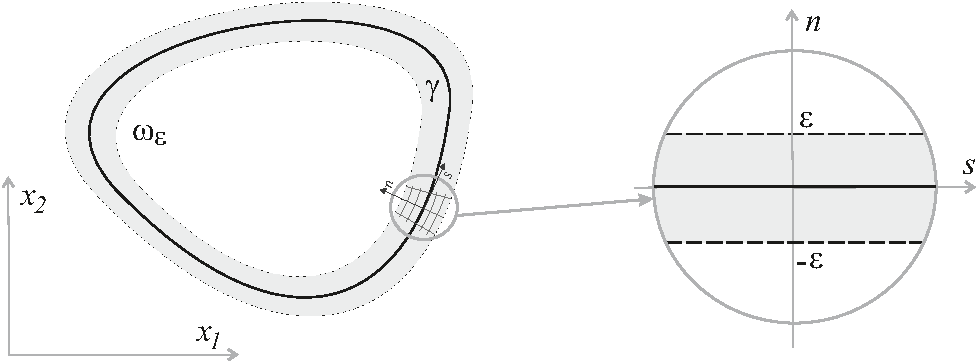
\includegraphics[scale=.6]{LocalCoords}
\caption{Curvilinear coordinates in the $\eps$-neighbourhood of $\gamma$.}
\label{FigLocalCoords}
\end{figure}


The family of potentials $V_\eps$ generally diverges in the space of distributions $\mathcal{D}(\Real^2)$.
As we will show  in Propositin~\ref{PropVepsConverg},
the  potentials converge only if $V$ is a zero mean function. In this case,
$V_\eps\to a \partial_\nu\delta_\gamma+b\delta_\gamma$ as $\eps\to 0$ for some functions $a$ and $b$,
where $\delta_\gamma$ is the Dirac delta function supported on $\gamma$ and $\partial_\nu\delta_\gamma$ is the normal derivative of $\delta_\gamma$ at points of $\gamma$. More precisely,
\begin{equation*}
  \langle a\partial_\nu\delta_\gamma+b \delta_\gamma, \phi \rangle= -\int_\gamma  \npt(a\phi)\,d\gamma+\int_\gamma b \phi\,d\gamma
\end{equation*}
for all $\phi\in C^\infty_0(\Real^2)$.



The main task is to construct asymptotic approximations, as $\eps\to 0$, to eigenvalues  and eigenfunctions of $H_\eps$, i.e., asymptotics of eigenvalues $\lambda^\eps$ and eigenfunctions $u_\eps$ of spectral equation
\begin{equation}\label{SpectralEqn}
-\Delta u_\eps +(W+V_\eps) u_\eps= \lambda^\eps u_\eps\quad \hbox{in \ } \Real^2.
\end{equation}





We  introduce some notation. The plane is divided into two domains by close curve $\gamma$.  We suppose that $\Real^2\setminus\gamma=\Omega_{in}\cup\Omega_{out}$, where domain $\Omega_{out}$ is unbounded. Also, we say that $v$ belongs to space $\mathcal{V}\subset L_2(\Real^2)$ if $v|_{\Omega_-}\in W_2^2(\Omega_{in})$ and there exist a function $w$ belonging to $\dom H_0$ such that $v=w$ in $\Omega_{out}$. Of course, $v|_{\Omega_{out}}\in W_{2,loc}^2(\Omega_{out})$.
Let $\mathcal{V}_0$ be the subspaces of $L_2(\Omega_{out})$
obtained by the restriction of all elements of $\mathcal{V}$ to $\Omega_{out}$.   We introduce two operators
\begin{align*}
&\mathcal{D}_1= -\Delta+W, \qquad \dom \mathcal{D}_1=\{v\in \mathcal{V}_0\colon\; v=0 \;\,\mbox{on } \gamma\},\\
&\mathcal{D}_2= -\Delta+W, \qquad \dom \mathcal{D}_2=\{v\in W_2^2(\Omega_{in})\colon\; v=0 \;\,\mbox{on } \gamma\}.
\end{align*}


We also denote by $\gamma_t=\{x\in\Real^2\colon\; x=\alpha(s)+t\nu(s), \; s\in S\}$ the closed curve that is obtained from $\gamma$ by flowing for ``time'' $t$ along the normal vector field. Then the boundary of $\omega_\eps$ consists of two curves $\gamma_{-\eps}$ and $\gamma_{\eps}$. For each $u\in \mathcal{V}$ there exist two one-side traces on $\gamma$, namely
\begin{equation}\label{UpmNotation}
  u^-=\lim_{\eps\to 0}u|_{\gamma_{-\eps}}, \qquad
u^+=\lim_{\eps\to 0}u|_{\gamma_{\eps}}.
\end{equation}







We say that the Schr\"odinger operator~$-\frac{d^2}{d t^2}+V$ in $L_2(\Real)$ possesses a \emph{zero-energy resonance}  if there exists a non trivial solution~$h$ of the equation $-h'' +Vh= 0$ that is bounded on the whole line.  We call $h$ the \emph{half-bound state} of $V$.  Such a solution~$h$ is  unique up to a scalar factor and has nonzero limits
\begin{equation*}
  h(-\infty)=\lim\limits_{t\to-\infty}h(t), \qquad
  h(+\infty)=\lim\limits_{t\to+\infty}h(t)
\end{equation*}
at both the infinities. We set
\begin{equation}\label{Theta}
  \theta=\frac{h(+\infty)}{h(-\infty)}.
\end{equation}



Our main result reads as follows.


\begin{thm}\label{MainThrm}
Let $W\in L^\infty_{loc}(\Real^2)$ and  $\dom H_0\subset W_2^1(\Real^2)$.
Assume  that potentials $V$ and $U$  are measurable bounded functions and assumption \eqref{pdsU} and \eqref{Vzeromean}  holds.
Then the family of operators
\begin{equation*}
 H_\eps=-\Delta +W+V_\eps,
\end{equation*}
where the perturbation $V_\eps$ is given by \eqref{Veps},
converges as $\eps\to 0$ in the strong resolvent sense.

If potential $V$ possesses a zero-energy resonance with a half-bound state $h$, then operators $H_\eps$ converge to  operator $\mathcal{H}$
defined by
$
\mathcal{H} v=-\Delta v+Wv
$
on functions $v\in \mathcal{V}$  obeying the interface conditions
\begin{equation}\label{ConnectedCond}
 u^+-\theta u^-=0,\quad  \theta\partial_\nu u^+-\partial_\nu u^-
=\left(\textstyle\frac{1}{2 }(\theta^2-1)\kappa+\mu\right) u^-
\end{equation}
on curve $\gamma$. Here  $\theta$ is given by  \eqref{Theta},  $\kappa$ is the signed curvature of $\gamma$, and
\begin{equation}\label{Mu}
  \mu=\frac{1}{h^2(-\infty)} \int_{\cI} U(\,\cdot\,,t)h^2(t)\, dt.
\end{equation}


If potential $V$ has no zero-energy resonance, then operators $H_\eps$ converge to the direct sum $\mathcal{D}_1\oplus\mathcal{D}_2$ of two unperturbed operators $-\Delta +W$ in $\Omega_{in}$ and $\Omega_{out}$ respectively with the Dirichlet boundary conditions on interface $\gamma$.
\end{thm}


\begin{rem}
  If potential $V$ is identically zero, then $V_\eps=\eps^{-1}\,U\left(s,\eps^{-1}n\right)$ and so obviously
$V_\eps\to \mu_0 \delta_\gamma$, as $\eps\to 0$, in the space of distributions. Here
\begin{equation}\label{Mu0}
  \mu_0(s)=\int_{\cI}U(s,t)\, dt.
\end{equation}
Potential $V=0$ possesses a zero-energy resonance with constant functions as  half-bound states. Hence parameter $\theta$ equals  $1$ and interface conditions \eqref{ConnectedCond} become
$ u^+- u^-=0$,  $\partial_\nu u^+-\partial_\nu u^-
-\mu_0 u^-=0$. These conditions are exactly the same as that obtained in \cite{BehrndtExnerHolzmannLotoreichik2017}.
\end{rem}






%%%%%%%%%%%%%%%%%%%%%%%%%%%%%%%%%%%%%%%%%%%%%%%%%%%%%%%%%%%%%%%%%%%%%%%%%%
% Preliminaries
%%%%%%%%%%%%%%%%%%%%%%%%%%%%%%%%%%%%%%%%%%%%%%%%%%%%%%%%%%%%%%%%%%%%%%%%%%

\section{Preliminaries}

Returning now to curvilinear coordinates $(s,r)$ given by \eqref{LocalTr},
we see that the couple of vectors
$ \tau=(\dot{\alpha}_1, \dot{\alpha}_2)$, $\nu=(-\dot{\alpha}_2, \dot{\alpha}_1)$
gives a Frenet frame for $\gamma$.
The Jacobian of transformation $x=\alpha(s)+r\nu(s)$ has the form
\begin{multline*}
J(s,r)=
\begin{vmatrix}
  \dot{\alpha}_1(s)-r\ddot{\alpha}_2(s)& -\dot{\alpha}_2(s)\\
          \dot{\alpha}_2(s)+r\ddot{\alpha}_1(s)\phantom{0} & \dot{\alpha}_1(s)
\end{vmatrix}
\\
=\dot{\alpha}_1^2(s)+\dot{\alpha}_2^2(s)
-r\big(\dot{\alpha}_1(s)\ddot{\alpha}_2(s)-
  \dot{\alpha}_2(s)\ddot{\alpha}_1(s)\big)=1-r \kappa(s).
\end{multline*}
Here $\kappa=\det(\dot{\alpha},\ddot{\alpha})$ is the signed curvature of $\gamma$. Note that $\kappa$ is a continuous function
of the arc-length parameter $s$ and the sign of $\kappa(s)$ is defined uniquely up to the re-parametrization $s\mapsto-s$.
We see that $J$ is positive for sufficiently small $n$, because  curvature $\kappa$  is  bounded on $\gamma$.
Namely, the curvilinear coordinates $(s,r)$ can be defined correctly on all domains $\omega_\eps$ with $\eps\leq \eps_*$, where
$\eps_*=\min_{\gamma}|\kappa|^{-1}$.
%However, the above we have accepted that $\eps_*=1$, since this
%involves no loss of generality.
We also have
\begin{equation}\label{IntegralCh}
  \int_{\omega_\eps} f(x_1,x_2)\,dx_1dx_2=\int_{Q_\eps} f(s,r)(1-r\kappa(s))\,ds\,dr
\end{equation}
for all integrable functions $f$.
The metric tensor $g=(g_{ij})$ of $\omega_\eps$ in the orthogonal coordinates $(s,r)$  has the form
  \begin{equation*}
    g=
    \begin{pmatrix}
      J^2\phantom{0} & 0 \\
          0\phantom{0} & 1
    \end{pmatrix}.
  \end{equation*}
In fact, we have
$g_{11}=|x_s|^2=|\dot{\alpha}+r \dot{\nu}|^2
=|(1-r\kappa) \dot{\alpha}|^2=J^2$,
by the Frenet-Serret formula $\dot{\nu}=-\kappa \dot{\alpha}$, and $g_{22}=|x_r|^2=|\nu|^2=1$.
In particular,  the gradient in the local coordinates becomes
\begin{equation*}
 \nabla \phi=\frac1{\sqrt{g_{11}}}\,\partial_s\phi\, \tau+\frac1{\sqrt{g_{22}}}\,\partial_r\phi\, \nu=\frac1J\,\partial_s\phi\, \tau+\partial_r\phi\, \nu
\end{equation*}
and  therefore we have
\begin{equation}\label{ScalarProdGrads}
  \nabla \phi\cdot \nabla \psi=J^{-2}\partial_s\phi\, \partial_s \psi+
\partial_r \phi\; \partial_r \psi.
\end{equation}
The Laplace-Beltrami operator in $\omega_\eps$ has also the explicit form
\begin{equation}\label{LaplacianInSN}
\Delta \phi=J^{-1}\left(\partial_s(J^{-1}\partial_s \phi)+ \partial_r(J\partial_r \phi)\right)
\end{equation}
as is easy to check.

Interface conditions \eqref{ConnectedCond} contain the parameters which depend on the particular parametrization chosen for curve $\gamma$. More precisely, parameters $\theta$, $\kappa$ and $\mu$ change along with the change of the Frenet frame.

\begin{prop}\label{PropInvarianceOfCnds}
  Operator $\mathcal{H}$ in Theorem~\ref{MainThrm} does not depend upon the choice of the Frenet frame for curve $\gamma$.
\end{prop}
\begin{proof}
Every smooth curve in the plane admits two possible orientations of arc-length parameter and consequently two possible  Frenet frames. Let us change the Frenet frame $\{\tau, \nu\}$, previously introduced in Sec.~\ref{Sec:Statment}, to the frame $\{-\tau, -\nu\}$ and prove that
interface conditions \eqref{ConnectedCond} will remain the same. This change leads to the following transformations:
\begin{gather*}
h(\pm\infty)\mapsto h(\mp\infty), \quad u_\pm\mapsto u_\mp, \quad \partial_\nu u_\pm \mapsto -\partial_\nu u_\mp,\\
\theta\mapsto \theta^{-1}, \quad \kappa\mapsto -\kappa,\quad \mu\mapsto \theta^{-2}\mu.
\end{gather*}
The first condition $u^+-\theta u^-=0$ in \eqref{ConnectedCond} transforms into $u^--\theta^{-1} u^+=0$ and therefore remains unchanged. As for the second condition, we have
\begin{equation*}
 	-\theta^{-1}\partial_\nu u^-+\partial_\nu u^+
	-\left(-\textstyle\frac{1}{2}(\theta^{-2}-1)\kappa
	+\theta^{-2}\mu\right) u^+=0.
\end{equation*}
Multiplying the equality by $\theta$  yields
\begin{equation*}
	\theta\partial_\nu u^+-\partial_\nu u^-
	-\left(\textstyle\frac{1}{2 }(\theta^{2}-1)\kappa+\mu\right) 	\theta^{-1} u^+=0,
\end{equation*}
since $-\theta(\theta^{-2}-1)=\theta^{-1}(\theta^{2}-1)$. It remains to insert $u^-$ in place of $\theta^{-1} u^+$, in view of the first interface condition.
\end{proof}

In the sequel, the normal vector field $\nu$ will be outward to domain $\Omega_{in}$, that is to say, the local coordinate $n$ will increase in the direction from $\Omega_{in}$ to $\Omega_{out}$.



%
%Notwithstanding the title of paper, all results presented in the article concern the potentials $V_\eps$ with arbitrary functions $V$ and $U$ of compact support, and $V_\eps$ generally diverge in the distributional sense. Therefore
%the $(a \partial_\nu\delta_\gamma+b\delta_\gamma)$-like potentials are only a partial case in our considerations. However,
%surprisingly enough, without reference to the convergence of $V_\eps$  the limit of $H_\eps$ exists in the strong resolvent sense. It is also worth noting that the convergence conditions for potentials $V_\eps$ and operators $H_\eps$ are quite different. In particular, the convergence of potentials does not depend on the existence of zero-energy resonances for $V$.


\begin{prop}\label{PropVepsConverg}
If $\int_\Real V\,dt=0$, then
\begin{equation*}
   V_\eps\to \beta\partial_\nu\delta_\gamma+\left(\beta\kappa+\mu_0\right) \delta_\gamma,\quad \mbox{as } \eps\to 0,
\end{equation*}
in the space of distributions $\mathcal{D}'(\Real^2)$, where
$\beta=-\int_\Real t V(t)\,dt$ and $\mu_0$ is given by \eqref{Mu0}.
\end{prop}
\begin{proof}
It is evident that potentials $\eps^{-1}\,U\left(s,\eps^{-1}r\right)$
converge to $\mu_0 \delta_\gamma$ in $\mathcal{D}(\Real^2)$.
We will prove that sequence $g_\eps=\eps^{-2}\,V\left(\eps^{-1}r\right)$ converges to
$\beta\left(\partial_\nu\delta_\gamma+\kappa\delta_\gamma\right)$ as $\eps\to 0$, provided $V$ is a zero-mean function.
In fact, for all $\phi\in C^\infty_0(\Real^2)$ we have
\begin{multline*}
\langle g_\eps, \phi \rangle=\int_{\omega_\eps}g_\eps(x)\phi(x)\,dx
=
\frac{1}{\eps^2}\int_{Q_\eps} V\left(\frac{r}{\eps}\right)\phi(s,r)(1-r\kappa(s))\,ds\,dr
\\
 =
\frac{1}{\eps}\int_{Q_1} V(t)\phi(s,\eps t)(1-\eps t\kappa(s))\,ds\,dt
\\
=\frac{1}{\eps}\int_{-1}^1 V(t)\,dt \int_S\phi(s,0)\,ds
\\
+
\int_{-1}^1 t V(t)\,dt \int_S\big(\partial_n\phi(s,0)-\kappa(s)\phi(s,0)\big)\,ds+O(\eps),
\end{multline*}
as $\eps\to 0$.
The sequence $\langle g_\eps, \phi \rangle$ has a finite limit for all $\phi\in C^\infty_0(\Real^2)$ if and only if $\int_\Real V\,dt=0$.
In this case, we have
\begin{equation*}
\langle g_\eps, \phi \rangle\to \beta\int_\gamma\left(\partial_\nu\delta_\gamma+\kappa \delta_\gamma\right)\phi\,d\gamma,
\end{equation*}
which completes the proof.
\end{proof}

\rd{At the end of the section},  we record some technical assertion, which  will be often used below.


%%%%%%%%%%%%%%%%%%%%%%%%%%%%%%%%%%%%%%%%%%%%%%%%%%%%%%%%%%%%%%%%%%%%%%%%%%
% Calculation of Limit Operator
%%%%%%%%%%%%%%%%%%%%%%%%%%%%%%%%%%%%%%%%%%%%%%%%%%%%%%%%%%%%%%%%%%%%%%%%%%

\section{Formal Asymptotics}
\subsection{Leading Terms}
\label{Sec:LimitOperator}

In this section we will show how interface conditions \eqref{ConnectedCond} can be found by direct calculations, constructing the formal asymptotics of  eigenvalues and eigenfunctions.
We  look for asymptotics of $\lambda_\eps$ and $u_\eps$ in the form
\begin{equation}\label{AsymptoticsUe}
\lambda^\eps\approx \lambda+\eps \lambda_1, \qquad u_\eps(x)\approx
\begin{cases}
  u(x)+\eps u_1(x)& \hbox{in \ }\Real^2\setminus \omega_\eps, \\
    v_0\left(s,\nep\right)+\eps v_1\left(s,\nep\right)+\eps^2 v_2\left(s,\nep\right)
&\hbox{in \ } \omega_\eps.
\end{cases}
\end{equation}
Recall that the boundary of $\omega_\eps$ consists of  two curves
$\gamma_{-\eps}$ and $\gamma_{\eps}$.
To match two different approximations, we hereafter assume that
\begin{equation}\label{MatchingCnds}
  [u_\eps]_{\gamma_{\pm\eps}}=0, \quad [\partial_\nu u_\eps]_{\gamma_{\pm\eps}}=0,
\end{equation}
where $[\,\cdot\,]_{\gamma_{\pm\eps}}$ is a jump  across $\gamma_{\pm\eps}$.
Since function $u_\eps$ solves \eqref{SpectralEqn} and domain $\omega_\eps$ shrinks to $\gamma$, the leading term $u$ must be a solution of the equation
\begin{equation*}
-\Delta u+Wu= \lambda u \quad \hbox{in \ } \Real^2\setminus \gamma,
\end{equation*}
subject to appropriate interface conditions on $\gamma$.
To find these conditions, we consider equation \eqref{SpectralEqn} in the curvilinear coordinates $(s,n)$, where $n=r/\eps$. Then in vicinity of $\gamma$ the Laplacian can be written as
\begin{equation}
  \Delta =\frac1{1-\eps n\kappa}\left( \eps^{-2}\partial_n
  (1-\eps n\kappa)\partial_n +\partial_s
  \Big(\frac1{1-\eps n\kappa}\,\partial_s\Big)\right),
\end{equation}
by \eqref{LaplacianInSN}.
From this we readily deduce the asymptotic representation
\begin{equation*}
\Delta= \eps^{-2}\partial^2_n-\eps^{-1}\kappa\partial_n
-n\kappa^2\partial_n+\partial^2_s+\eps P_\eps,
\end{equation*}
where $P_\eps$ is a partial differential operator on the second order with respect to $s$ and the first one with respect to $n$ whose coefficients  are uniformly bounded on $\eps$.
Substituting \eqref{AsymptoticsUe} into \eqref{SpectralEqn} for $x\in \omega_\eps$ in particular yields
\begin{equation}\label{EqnsV0V1}
-\pte^2 v_0+V(n)v_0=0,
\qquad
-\pte^2 v_1+V(n)v_1=-\kappa(s)\pte v_0-U(s,n)v_0
\end{equation}
in cylinder $Q_1=S\times(-1,1)$.
From \eqref{MatchingCnds} we see that necessarily
\begin{gather}\label{FittingCndsUV0}
 u^-(s)=v_0(s,-1),\qquad u^+(s)=v_0(s,1),
 \\\label{FittingCndspV0}
 \partial_n v_0(s,- 1)=0, \qquad \partial_n v_0(s, 1)=0, \\\label{FittingCndspV1}
 \partial_n v_1(s, -1)=\partial_\nu u^-(s), \qquad
 \partial_n v_1(s, 1)=\partial_\nu u^+(s),
\end{gather}
where $u^\pm$ are defined by \eqref{UpmNotation}.
Combining \eqref{FittingCndspV0}--\eqref{FittingCndspV1}, we conclude that $v_0$ and $v_1$ solve boundary value problems
\begin{align}\label{problemV0}
&\begin{cases}
  -\pte^2 v_0+V(n)v_0=0 \quad \hbox{in \ } Q_1, \\
    \phantom{-}\partial_n v_0(s,- 1)=0, \quad \partial_n v_0(s, 1)=0, \quad s\in S;
\end{cases}
\\\label{problemV1}
&\begin{cases}
  -\pte^2 v_1+V(n)v_1=-\kappa(s)\pte v_0-U(s,n)v_0\quad \hbox{in \ } Q_1, \\
    \phantom{-}\partial_n v_1(s, -1)=\partial_\nu u^-(s), \quad
\partial_n v_1(s, 1)=\partial_\nu u^+(s), \quad s\in S
\end{cases}
\end{align}
respectively.
We have two boundary value problems for the ``non-ellip\-tic'' partial differential operator in $Q_1$. Of course,  the problems can also be  regarded as  boundary value problems for ordinary differential equations on $(-1,1)$, which depend on parameter $s\in S$.



%
%In fact, let $\ell$ be the length of $S$ and then the length of $\gamma$. Then both problems \eqref{problemV0} and  \eqref{problemV1} can write out as  boundary value problem in  rectangle $\Pi=(0,\ell)\times(-1,1)$
%\begin{equation*}
%  \begin{cases}
%    -\pte^2 v+V(t)v=g(s,n), \qquad (s,n)\in \Pi, \\
%    \phantom{-}\partial_t v(s,- 1)=a_-(s), \quad \partial_t v(s, 1)=a_+(s), \quad s\in S,\\
%\phantom{-}v(0,t)=v(\ell,t), \quad \partial_s v(0,t)=\partial_s v(\ell,t), \quad t\in (-1,1)
%  \end{cases}
%\end{equation*}
%with the Neumann boundary conditions with respect to $t$ and the periodicity conditions with respect to $s$.
%In any case, the lack of ellipticity  leads to a loss of smoothness of solutions with respect to $s$, and this will have an considerable influence on the proof of Theorem~\ref{MainThrm}.
%



















\textit{Case of zero-energy resonance.}
Assume that operator $-\frac{d^2}{dt^2}+V$ has a zero energy resonance with half-bound state $h$. Since the support of $V$ lies in  interval $(-1,1)$, the half-bound state $h$ is  constant  outside this interval as a bounded solution of equation $h''=0$.
Therefore the restriction of $h$ to $(-1,1)$ is a nonzero solution of the Neumann boundary value problem
\begin{equation}\label{NeumanProblem}
     -h''+V(n)h= 0,\quad n\in(-1,1),\qquad   h'(-1)=0, \quad h'(1)=0.
\end{equation}
Hereafter, we fix $h$ by additional condition $h(-1)=1$. In view of
\eqref{Theta}, we have $h(1)=\theta$, since $h(\pm\infty)=h(\pm 1)$.




In this case, \eqref{problemV0}  admits a infinite-dimensional space of solutions
\begin{equation*}
\mathcal{N}=\big\{a(s)h(n)\colon \;a\in L^2(S)\big\}.
\end{equation*}
Therefore $v_0(s,n)=a_0(s)h(n)$ for some function $a_0$. From \eqref{FittingCndsUV0} we deduce that $u^-=a_0$ and $u^+=\theta a_0$ and hence that
\begin{equation}\label{RCond0}
     u^+=\theta u^-\quad\text {on }\gamma.
\end{equation}
In addition, we must set $v_0(s,n)=u^-(s)h(n)$.


Problem \eqref{problemV1} is in general unsolvable, since $\mathcal{N}\neq\{0\}$.  To find solvabi\-li\-ty conditions, we rewrite  equation in \eqref{problemV1} as
\begin{equation}\label{eqnV1Expand}
  -\pte^2 v_1+V(n)v_1=-\big(\kappa(s)h'(n)+U(s,n)h(n)\big)u^-(s),
\end{equation}
multiply  by an arbitrary element of  $\mathcal{N}$  and then integrate over $Q_1$
\begin{multline}\label{IntV1H}
\int_{Q_1}\left(-\pte^2 v_1+V(n)v_1\right)a(s)h(n)\,dn\,ds
\\
=
-\int_{Q_1}(\kappa(s)h'(n)+U(s,n)h(n))u^-(s)a(s)h(n)\, dn\,ds.
\end{multline}
Since $h$ is a solution of \eqref{NeumanProblem}, integrating by parts twice on the left-hand side yields
\begin{multline*}
\int_{S} \int_{-1}^1\left(-\pte^2 v_1+Vv_1\right)a h\,dn \,ds
=-\int_{S}( \partial_n v_1 h-v_1 h')\big|_{n=-1}^{n=1}a\,ds\\-
\int_{S} \int_{-1}^1 a v_1\left(-h''+Vh\right)\,dn\,ds
=-\int_{S}\big(\theta\partial_\nu u^+-\partial_\nu u^-\big) a\,ds,
\end{multline*}
in view of the boundary conditions for $v_1$.
Recall that $h(-1)=1$ and $h(1)=\theta$.
Since $hh'=\frac12 (h^2)'$, we also have $\int_{-1}^1hh'\,d t=\textstyle\frac{1}{2 }(\theta^2-1)$.
Therefore \eqref{IntV1H} becomes
\begin{equation*}
\int_{S}\left(\theta\partial_\nu u^+-\partial_\nu u^-\right)a\,ds
=\int_{S}\big(\textstyle\frac{1}{2}(\theta^2-1)\kappa+\mu \big)u^-a\,ds
\end{equation*}
for all  $a\in L^2(S)$, where $\mu(s)=\int_{-1}^1 U(s,n)h^2(n)\, dn$.
Therefore
\begin{equation*}
  \theta\partial_\nu u^+-\partial_\nu u^-
=\big(\textstyle\frac{1}{2}(\theta^2-1)\kappa+\mu \big) u^-\quad\text {on }\gamma,
\end{equation*}
which is necessary for the solvability of \eqref{problemV1}.
In view of the Fredholm alternative, this condition is also a sufficient one. At the same time, it is a jump condition at the interface $\gamma$ for the normal derivative of $u$.

Therefore the leading terms $\lambda$ and $u$ of asymptotics \eqref{AsymptoticsUe} solve the problem
\begin{gather}\label{LimitProblemEq}
-\Delta u+Wu=\lambda u \qquad \hbox{in  } \Real^2\setminus \gamma,
\\ \label{RConds}
 \phantom{-}u^+-\theta u^-=0,  \quad
\theta\partial_\nu u^+-\partial_\nu u^-
=\big(\textstyle\frac{1}{2}(\theta^2-1)\kappa+\mu \big) u^- \quad \hbox{on } \gamma.
\end{gather}
Assume that $\lambda$ is an eigenvalue of operator $\cH$ associated with the eigenfunction~$u$. Now we can calculated the trace $u^-$ on $\gamma$ and  finally determine $v_0(s,n)=u^-(s)h(n)$.

\textit{Non-resonant case.}
Now suppose that problem \eqref{NeumanProblem} admits the trivial solution only, i.e.,  $\mathcal{N}=\{0\}$.  Then $v_0=0$ and therefore $u^-=0$ and $u^+=0$ on $\gamma$, by \eqref{FittingCndsUV0}. We thus get
\begin{equation*}
-\Delta u+Wu=\lambda u\quad \hbox{in \ } \Real^2\setminus \gamma,\qquad
 u|_{\gamma}=0.
\end{equation*}
Let us suppose that $\lambda$ is an eigenvalue of the direct sum
$\mathcal{D}_1\oplus\mathcal{D}_2$ of two Dirichlet type operators and $u$ is a corresponding eigenfunction.
In this case, problem \eqref{problemV1} has the form
\begin{equation}\label{problemV1Non}
\begin{cases}
    -\pte^2 v_1+V(n)v_1=0\quad \hbox{in \ } Q_1, \\
    \phantom{-}\partial_n v_1(s, -1)=\partial_\nu u^-, \qquad
\partial_n v_1(s, 1)=\partial_\nu u^+,
\end{cases}
\end{equation}
and admits a unique solution.

\section{Proof of Main Theorem}
Let $\{\lambda^\eps\}_{\eps>0}$ be a sequence of eigenvalues of operator $H_\eps$ and $\{u_\eps\}_{\eps>0}$ be the sequence of the corresponding eigenfunctions. Assume that $\|u_\eps\|_{L_2(\Real^2)}=1$.


\begin{lem}\label{lemConvD}
  Suppose that $\lambda^\eps\to \lambda$ and $u_\eps\to u$ in $L_2(\Real^2)$ weakly as $\eps\to 0$. Then $u_\eps$ converge to $u$ in the $L_2(\Real^2)$-norm. Moreover, if the one-dimensional Schr\"odinger operator~$-\frac{d^2}{d t^2}+V$  possesses a zero-energy resonance, then $\lambda$ is an eigenvalue of $\cH$ associated with the eigenfunction $u$. Otherwise $\lambda$ is an eigenvalue and $u$ is the corresponding eigenfunction  of the direct sum $\mathcal{D}_1\oplus\mathcal{D}_2$.
\end{lem}


We have divided the proof into a sequence of propositions.

\begin{prop}
  Under the assumptions of Lemma~\ref{lemConvD}, for every $\beta>0$ the sequence $u_\eps$ converges to $u$ in $W_2^2(\Real^2\setminus \omega_\beta)$ weakly and $u$ solves the equation
  \begin{equation*}
    -\Delta u+Wu=\lambda u \quad \text{in  } \Real^2\setminus \gamma.
  \end{equation*}
 In addition,  $u_\eps|_{\gamma_{-\eps}}\to u^-$ and $u_\eps|_{\gamma_{\eps}}\to u^+$ in $L_2(\gamma)$ weakly as $\eps\to 0$, where $u^\pm$ are given by \eqref{UpmNotation}.
\end{prop}
\begin{proof}
  Let $\Phi_\gamma$ be the set of test functions $\phi\in C_0^\infty(\Real^2)$ such that $\phi=0$ in $\omega_\beta$. We conclude from \eqref{SpectralEqn} that
  \begin{equation}\label{DeltaUconv}
    \int_{\Real^2} \Delta u_\eps\phi\,dx=\int_{\Real^2} (W-\lambda^\eps)\,u_\eps\phi\,dx, \quad\phi\in \Phi_\beta,
  \end{equation}
for all $\eps<\beta$, since the support of short-range potential $V_\eps$ lies in $\omega_\beta$. The right-hand side of \eqref{DeltaUconv} has a limit as $\eps\to 0$ by the assumptions, thus the left-hand side also converges for all $\phi\in \Phi_\beta$, i.e., $\Delta u_\eps\to \Delta u$ in $L_2(\Real^2)$ weakly. From this we deduce that $u_\eps$ converges to $u$ in  $W_2^2(\Real^2\setminus \omega_\beta)$ weakly, and hence that
  \begin{equation}\label{DeltaUconv}
    \int_{\Real^2} \Delta u\phi\,dx=\int_{\Real^2} (W-\lambda)\,u\phi\,dx, \quad\phi\in \Phi_\beta.
  \end{equation}
So $u$ is a solution of the equation  $-\Delta u+Wu=\lambda u$
in $\Real^2\setminus \omega_\beta$  and, therefore,  in $\Real^2\setminus \gamma$,
since $\beta$ is an arbitrary positive number.

\begin{figure}[b]
  \centering
  % Requires \usepackage{graphicx}
  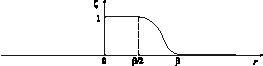
\includegraphics[scale=1.8]{JumpFunction}\\
  \caption{Plot of the function $\zeta$.}\label{FigPlotZeta}
\end{figure}

The function $\zeta$  is as shown in Fig.~\ref{FigPlotZeta}. In particular, $\zeta$ is smooth outside the origin,  $\zeta(r)=1$ for $r\in (0,\beta/2)$ and $\zeta(r)=0$ in the set $\Real\setminus [0,\beta]$.
Let $\chi_\eps$ be the characteristic function of the set $(\eps,+\infty)$.
We introduce the function
$$
\zeta_\eps(r)=(r-\eps)\zeta(r)\chi_\eps(r).
$$
Since $\zeta_\eps(\eps)=0$ and $\zeta_\eps'(\eps+0)=1$ for $\eps<\beta/2$, we readily deduce  the equality
\begin{equation}\label{IntUepsDg}
  \int_{\gamma_\eps} u_\eps a \,d\gamma=\int_{\Omega_{out}^\eps} (W-\lambda^\eps)u_\eps a\zeta_\eps\,dx-\int_{\Omega_{out}^\eps} u_\eps \Delta (a\zeta_\eps)\,dx,
\end{equation}
where $a$ is a smooth function on $\gamma$ and $\Omega_{out}^\eps=\Omega_{out}\setminus\omega_\eps$.
Similarly, we have
 \begin{equation}\label{IntUDg}
  \int_{\gamma} u^+ a \,d\gamma=\int_{\Omega_{out}} (W-\lambda)u^+ a\zeta_0\,dx-\int_{\Omega_{out}} u^+ \Delta (a\zeta_0)\,dx,
\end{equation}
where $\zeta_0(r)=r\zeta(r)$.
Obviously,
\begin{equation*}
   \int_{\Omega_{out}^\eps} (W-\lambda^\eps)u_\eps a\zeta_\eps\,dx\to
   \int_{\Omega_{out}} (W-\lambda)u^+ a\zeta_0\,dx
\end{equation*}
as $\eps\to 0$, because $\zeta_\eps$ converge to $\zeta_0$ uniformly on $\Real_+$. Recalling representation \eqref{LaplacianInSN} of the Laplace operator in the local coordinates, we can write
\begin{multline}\label{IntDelta}
  \int_{\Omega_{out}^\eps}u_\eps \Delta (a\zeta_\eps)\,dx=
  \int_{S} \int_0^\beta u_\eps(s,r)\rho_\eps(r) \,\partial_s\left(\frac{a'(s)}{1-r \kappa(s)}\right)\,ds\,dr
  \\
  +\int_{S} \int_0^\beta u_\eps(s,r)a(s)\big(J(s,r)(2\zeta'(r)+(r-\eps)\zeta''(r))
  -\kappa(s)(r-\eps)\zeta'(r)\big)\,ds\,dr\\
  -
  \int_{S} \int_\eps^\beta u_\eps(s,r)a(s)\kappa(s)\zeta(r)\,ds\,dr,
\end{multline}
provide $\eps<\beta/2$. Here we used  the equalities $\zeta'(r)=0$ and $\zeta''(r)=0$ for $r\in(0,\eps)$.
The right-hand side of \eqref{IntDelta} converges to
\begin{multline*}
   \int_{S} \int_0^\beta u^+(s,r)\rho_0(r) \,\partial_s\left(\frac{a'(s)}{1-r \kappa(s)}\right)\,ds\,dr
  \\
  +\int_{S} \int_0^\beta u^+(s,r)a(s)\big(J(s,r)(2\zeta'(r)+r\zeta''(r))
  -\kappa(s)(\zeta(r)+r\zeta'(r))\big)\,ds\,dr,
\end{multline*}
which coincides with $\int_{\Omega_{out}}u^+ \Delta (a\zeta_0)\,dx$.
Therefore we conclude from \eqref{IntUepsDg} and \eqref{IntUDg} that
$\int_{\gamma_\eps} u_\eps a \,d\gamma\to \int_{\gamma} u^+ a \,d\gamma$ for all $a\in C^\infty(\gamma)$, hence that  $u_\eps|_{\gamma_{\eps}}\to u^+$ in $L_2(\gamma)$ weakly as $\eps\to 0$. The proof of the weak convergence for   $u_\eps|_{\gamma_{-\eps}}$ is similar.
\end{proof}


The eigenvalue $\lambda^\eps$ and the corresponding eigenfunction $u_\eps$ satisfy the identity
\begin{equation*}
   \int_{\Real^2}\big(\nabla u_\eps \nabla \phi+
              (W+V_\eps-\lambda^\eps)u_\eps \phi\big)\,dx=0, \qquad \phi\in \dom H_0,
\end{equation*}
which may be rewritten as
\begin{equation}\label{IdentityUe}
   \int_{\omega_\eps}\big(\nabla u_\eps \nabla \phi+
   V_\eps u_\eps \phi\big)\,dx=
    -\int_{\Omega_\eps}\nabla u_\eps \nabla \phi\,dx- \int_{\Real^2}
              (W-\lambda^\eps)u_\eps \phi\,dx
\end{equation}
We denote by $\Omega_\eps$ the set $\Real^2\setminus\omega_\eps$. The right-hand side of \eqref{IdentityUe} has a finite limit
\begin{equation*}
  -\int_{\Real^2}\big(\nabla u \nabla \phi+
              (W-\lambda)u \phi\big)\,dx
\end{equation*}
as $\eps\to 0$. In particular, the term $\int_{\Real^2}Wu_\eps \phi\,dx$ converges  for any  $\phi\in \dom H_0$ by the rapidly decay of  eigenfunctions of $H_\eps$ \cite[Ch.3.3]{BerezinShubinBook}. Therefore the left-hand side of \eqref{IdentityUe} also converges as $\eps\to 0$.

\begin{prop}
  Suppose that operator $-\frac{d^2}{d t^2}+V$ possesses a zero-energy resonance with a half-bound state $h$. Then
  \begin{equation*}
    \int_{\omega_\eps}\big(\nabla u_\eps \nabla \phi+
   V_\eps u_\eps \phi\big)\,dx\to
\int_\gamma\left(\tfrac12(\theta^2-1)\kappa+\mu\right) u^-\phi\,d\gamma
  \end{equation*}
\end{prop}


Let $\lambda$ and $u$ the eigenvalue and the corresponding eigenfunction of
 $\cH$. Then
\begin{equation*}
   \int_{\Real^2}\big(\nabla u \nabla \psi+Wu\psi\big)\,dx
   +\int_\gamma\left(\tfrac12(\theta^2-1)\kappa+\mu\right) u^-\phi^-\,d\gamma=\lambda\int_{\Real^2}u \psi\,dx
\end{equation*}
for all functions $\psi$ belonging to the class $\Psi_\theta=\{\psi\in\cV\colon \psi^+=\theta \psi^-\text{ on }\gamma\}$.

We introduce the smoothing operator $R_\eps\colon \Psi_\theta\to \dom H_0$
as follows. Suppose that functions $h_0$, $h_1$ and $h_2$ solve the Cauchy problems on the interval $\cI$
\begin{align*}
&-h_0''+Vh_0=0,\quad  h_0(-1)=1, \quad h_0'(-1)=0;
\\
&-h_1''+Vh_1=0,\quad  h_1(-1)=0, \quad h_1'(-1)=1;
\\
&\begin{cases}
  -h_2''+Vh_2=\kappa(s)h'_0+U(s,\,\cdot\,)h_0,
  \\
\phantom{-}h_2(s,-1)=0, \quad \partial_n h_2(s,-1)=0,\quad s\in S
\end{cases}
\end{align*}
respectively.

Given any function $\psi\in\Psi_\theta$, let us set
\begin{equation*}
  \psi_{0,\eps}(s,n)=\psi(s,-\eps)\,h_0(n), \quad
  \psi_{1,\eps}(s,n)=\partial_\nu\psi(s,-\eps)\,h_1(n)
     -\psi(s,-\eps)\,h_2(s,n),
\end{equation*}
where





\begin{equation*}
  (R_\eps\psi)(x)=
  \begin{cases}
    \psi(x), & \text{if } x\in \Real^2\setminus \omega_\eps,\\
     \psi(s,-\eps)h_0(\tfrac{r}{\eps})
     +\eps\big(\partial_\nu\psi(s,-\eps)h_1(\tfrac{r}{\eps})
     -\psi(s,-\eps)h_2(s,\tfrac{r}{\eps})\big)
  \end{cases}
\end{equation*}











\begin{thebibliography}{10}
\bibitem{BehrndtExnerHolzmannLotoreichik2017}
Behrndt, J., Exner, P., Holzmann, M.,  Lotoreichik, V. (2017). Approximation of Schrodinger operators with $\delta$-interactions supported on hypersurfaces. Mathematische Nachrichten, 290(8-9), 1215-1248.


\bibitem{BerezinShubinBook} F. A. Berezin, M. A. Shubin,
\textit{The Schr\"{o}dinger equation.} Kluwer Academic
Publishers, 1991.

\bibitem{GolovatyHrynivJPA:2010}
    Yu. D. Golovaty,  R. O. Hryniv.
    \textit{On norm resolvent convergence of Schr\"{o}dinger
    operators with $\delta'$-like potentials.}
   Journal of Physics A: Mathematical and Theoretical \textbf{43} (2010) 155204 (14pp) (A Corrigendum: 2011 J. Phys. A: Math. Theor. \textbf{44} 049802)

\bibitem{Golovaty:2012}
    Yu.~Golovaty.
    \textit{Schr\"{o}dinger operators with  $(\alpha\delta'+\beta \delta)$-like potentials: norm resolvent convergence and solvable models,} Methods of Funct. Anal. Topology (3) \textbf{18} (2012), 243--255.

\bibitem{GolovatyHrynivProcEdinburgh2013} Yu. D. Golovaty and R. O. Hryniv. \textit{Norm resolvent convergence of singularly scaled Schr\"{o}dinger operators and $\delta'$-potentials.} Proceedings of the Royal Society of Edinburgh: Section A Mathematics \textbf{143} (2013),  791-816.

\bibitem{GolovatyIEOT2013}
    Yu. Golovaty, \textit{1D Schr\"{o}dinger Operators with Short Range Interactions: Two-Scale Regularization of Distributional Potentials.} Integral Equations and Operator Theory \textbf{75}(3) (2013),   341-362.


\bibitem{Zolotaryuk08}
    A. V. Zolotaryuk.
    \textit{Two-parametric resonant tunneling across the $\delta'(x)$ potential.}
    Adv. Sci. Lett. {\bf 1} (2008), 187-191.

\bibitem{Zolotaryuk09}
    A. V. Zolotaryuk.
    \textit{Point interactions of the dipole type defined through a three-parametric power regularization.}
    Journal of Physics A: Mathematical and Theoretical {\bf 43} (2010), 105302.

\bibitem{GolovatyJPA:2018}
	Yu. Golovaty.
	\textit{Two-parametric  $\delta'$-interactions: approximation by
 	Schr\"{o}dinger operators with localized rank-two perturbations.}
 	Journal of Physics A: Mathematical and Theoretical \textbf{51}(25) (2018), 255202.

\bibitem{GolovatyIEOT:2018}
	Yu. Golovaty.
	\textit{Schr\"{o}dinger operators with singular rank-two perturbations and point interactions.}
	Integr. Equ. Oper. Theory \textbf{90}:57 (2018).
\end{thebibliography}

\end{document}

We also have $v_0(s,t)=u^-(s)h(t)=\theta^{-1}u^+(s)h(t)$.
